\documentclass[dvipdfmx,tikz]{standalone}
\usepackage{tikz,bm,amsmath}
\begin{document}
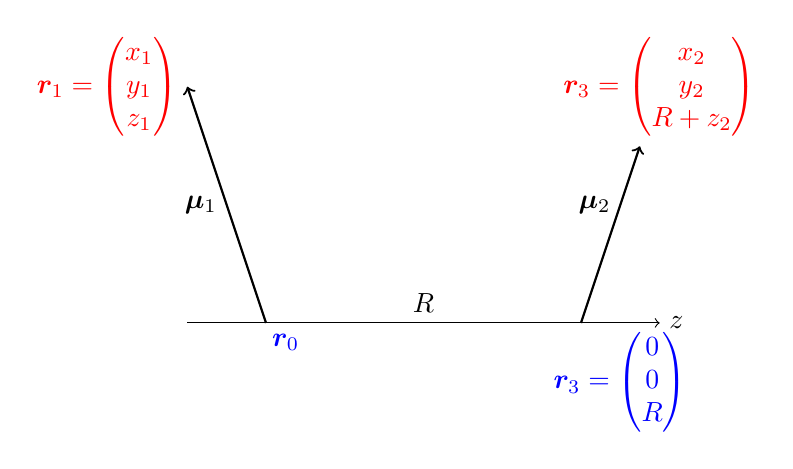
\begin{tikzpicture}
%\draw[help lines] (-1,-1) grid (4,1);
\draw[->] (-1,0) -- (5,0) node[anchor = west] {$z$};

\node[red,anchor=east] (q1+) at (-1,3) {$\bm{r}_1 = \begin{pmatrix}
    x_1 \\
    y_1 \\
    z_1
\end{pmatrix}$};
\node[blue] (q1-) at (0.25,-0.25) {$\bm{r}_0$};
\draw[->,thick] (0,0) -- (-1,3){};
\node[anchor=east] at (-0.5,1.5) {$\bm{\mu}_1$};

\node[red] (q2+) at (5,3) {$\bm{r}_3
=
\begin{pmatrix}
    x_2 \\
    y_2 \\
    R + z_2
\end{pmatrix}$};
\node[blue] (q2-) at (4.5,-0.75) {$\bm{r}_3
=
\begin{pmatrix}
    0 \\
    0 \\
    R
\end{pmatrix}$};
\draw[->,thick] (4,0) -- (q2+){};
\node[anchor=east] at (4.5,1.5) {$\bm{\mu}_2$};

\node[thick] at (2,0.25) {$R$};
\end{tikzpicture}
\end{document}